% !TeX root = ../main.tex

\chapter{龙芯安卓图形栈设计与实现}
本章将详细介绍在现有龙芯硬件平台下,安卓图形栈的设计与实现。首先是对图形系统进行分析,从整体架构上介绍图形系统的基本框架,包括安卓框架部分以及龙芯硬件
支持部分,以及如何在Android上支持LoongArch和LG110。之后介绍图形系统的四个主要组成部分:内核图形驱动模块,用户态图形驱动模块,安卓gralloc模块和硬件混合渲染(HWC)模块。内核驱动模块负责对接用户态驱动
和GPU固件之间的联系。用户态驱动负责向安卓框架提供龙芯硬件支持。而gralloc模块是根据龙芯硬件驱动向安卓上层libui库提供服务,硬件混合渲染(HWC)模块为安卓中进行窗口
(Layer)合成和显示的HAL模块。(标注:还需完善,暂且这样)

\section{硬件兼容性标准}
根据Android12的兼容性文档\cite{Android-12-cdd}中有关2D和3D图形加速的部分,对于硬件设备和配套驱动作出如下约束,必须支持OpenGL ES 1.1和2.0,以及如下10种拓展\ref{tab:Android12兼容拓展要求}。
\begin{table}[h]
  \centering
  \caption{Android12兼容拓展要求}
  \label{tab:Android12兼容拓展要求}
  \begin{tabular}{l}
    \toprule
    拓展名  \\
    \midrule
    EGL\_KHR\_image \\
    EGL\_KHR\_image\_base \\
    EGL\_ANDROID\_image\_native\_buffer \\
    EGL\_ANDROID\_get\_native\_client\_buffer \\
    EGL\_KHR\_wait\_sync \\
    EGL\_KHR\_get\_all\_proc\_addresses \\
    EGL\_ANDROID\_presentation\_time \\
    EGL\_KHR\_swap\_buffers\_with\_damage \\
    EGL\_ANDROID\_recordable \\
    EGL\_ANDROID\_GLES\_layers \\
    \bottomrule
  \end{tabular}
  \note{}
\end{table}
目前龙芯LG110及配套驱动均已满足相关最低兼容性要求标准,可以进行适配。
% \subsection{功能性需求}
% 1.龙芯硬件驱动接口的正确性
% 2.更多特性支持

% \subsection{非功能性需求}
% 1.兼容性
% 2.高效性
% 3.快速启动

\section{整体设计}
Android的图形系统作为安卓最复杂的模块之一,在开始移植的工作之前,首先需要对其整体结构做一个分析。为了兼容硬件供应商的不同的底层硬件实现,
安卓framework层定义了大量的抽象接口规定了每个安卓版本的所需实现的功能,而具体的功能实现则需要各家硬件供应商去实现。本节首先阐述安卓图形栈的整体结构,
分析Android 图形模块运行的关键,明确图形系统的方案,再对涉及到的部分关键流程进行说明。
\subsection{安卓图形系统的整体构成}
\begin{figure}[h]
  \centering
  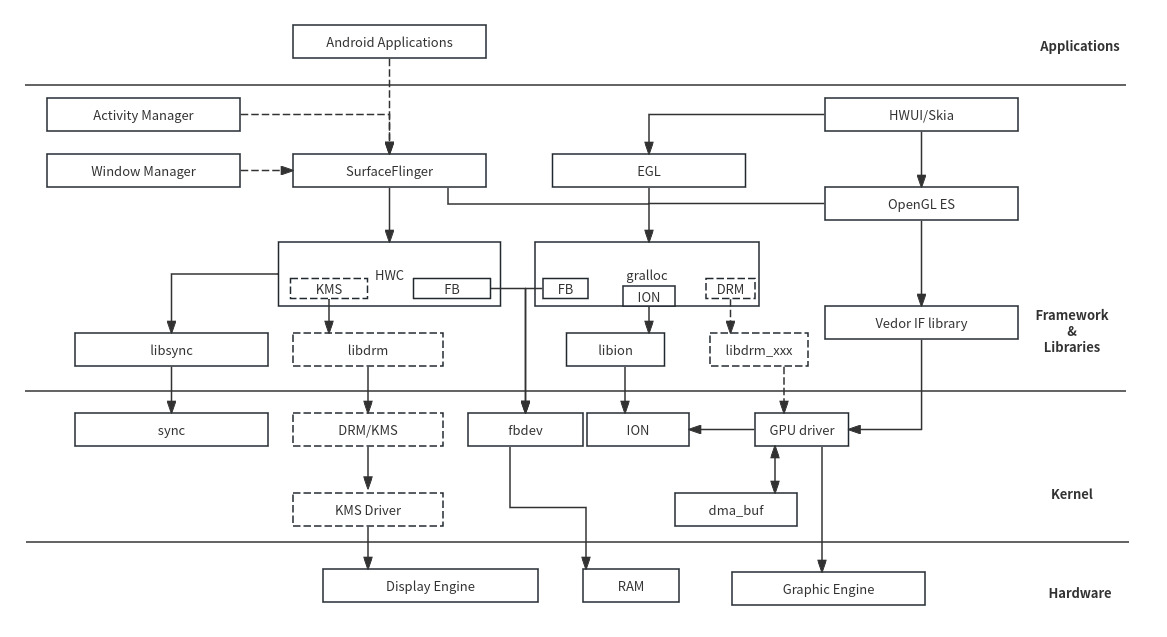
\includegraphics[width=0.8\textwidth]{安卓图形栈结构图.jpg}
  \caption{安卓图形栈结构图}    
  \label{fig:安卓图形栈结构图}
\end{figure}
自上往下分析,Android应用、活动管理器(Activity Manager)、窗口管理器(Window Manager)以及部分安卓Native程序(如BootAnimation)等首先与Surface进行交互,
根据自己的需求创建一个Surface,然后数个Surface会被SurfaceFlinger进行混合\cite{邓凡平2011深入理解}。
因此图形系统中最关键的服务进程就是SurfaceFlinger,负责管理图形缓冲区的合成与显示,如图\ref{fig:安卓图形栈结构图}所示,它将来自不同应用的图形缓冲区进行合成,
并将合成结果发送到显示设备。因此,图形系统的正确运行一个重要的环节就是确保SurfaceFlinger的正确运行。而SurfaceFlinger的运行依赖于硬件抽象层(HAL)和底层图形库。
这其中有两个重要的模块,一个是HWC(硬件混合渲染器),是进行窗口合成和显示HAL层模块,其实现是特定于设备的,通常是由显示设备制造商 (OEM)完成。其用于合成从Surfaceflinger接收
的图层,从而减少OpenGL ES (GLES) 和 GPU 执行的合成量。但是实际上由于LG110并不是专门为安卓平台设计的显卡,并没有实现硬件图层混合的功能,因此hwcomposer使用的是client合成模式,
也就是直接使用GPU的OpenGL ES实现进行合成。
另一个模块是gralloc。它是Android中负责申请和释放GraphicBuffer的HAL层模块,
由硬件驱动提供实现,为BufferQueue机制提供了基础。gralloc的主要组件包括Allocator,Mapper。Allocator 负责内存的分配和释放,
主要功能包括:根据请求的大小和格式分配内存缓冲区,负责跟踪已分配和空闲的内存块以及支持在多个进程之间共享缓冲区,使得不同的应用程序或组件能够访问同一块内存。
Mapper负责将已分配的缓冲区映射到进程的虚拟地址空间。本课题需要实现支持龙芯硬件平台的gralloc和HWC模块的库以支持SurfaceFlinger的正确运行。
\begin{figure}[h]
  \centering
  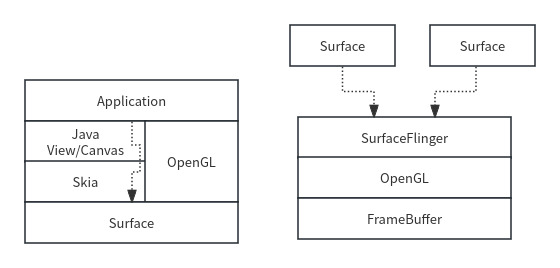
\includegraphics[width=0.8\textwidth]{Surface系统.jpg}
  \caption{Surface系统的任督二脉}    
  \label{fig:Surface系统的任督二脉}
  \cite{邓凡平2011深入理解}
\end{figure}

安卓的framework层以及库函数依赖的图形接口是由libdrm进行封装,包括上文提及的gralloc和HWC都是需要使用libdrm定义的接口。libdrm是一个用户态空间的库,
提供了与 Linux 内核中的 DRM(Direct Rendering Manager)子系统交互的接口。它是 Linux 图形栈的核心组件之一(同样也是Android图形栈的方案),
用于管理图形硬件资源(如 GPU、显示控制器和缓冲区),并支持硬件加速的图形渲染与显示。libdrm 通过封装 DRM 的 IOCTL 系统调用,
为用户空间程序(如显示服务器、图形驱动和应用程序)提供了简单易用的 API。
至于内核部分仍然是依赖linux内核的KMS和DRM。DRM/KMS 是 Linux 内核中用于管理图形硬件的子系统,提供了对 GPU、显示控制器和显示设备的统一抽象。在上层的系统级服务中,
SurfaceFlinger是通过HWC(Hardware Composer)与DRM/KMS交互,HWC负责将图形缓冲区合成任务委托给硬件。在 DRM/KMS 框架下,HWC 通过 DRM 接口与内核通信,
管理显示模式设置、缓冲区分配和显示同步等任务。KMS 负责配置显示控制器和显示设备的分辨率、刷新率等参数,而 DRM 则管理图形缓冲区的分配与渲染。

\subsection{关键流程分析}
\begin{figure}[h]
  \centering
  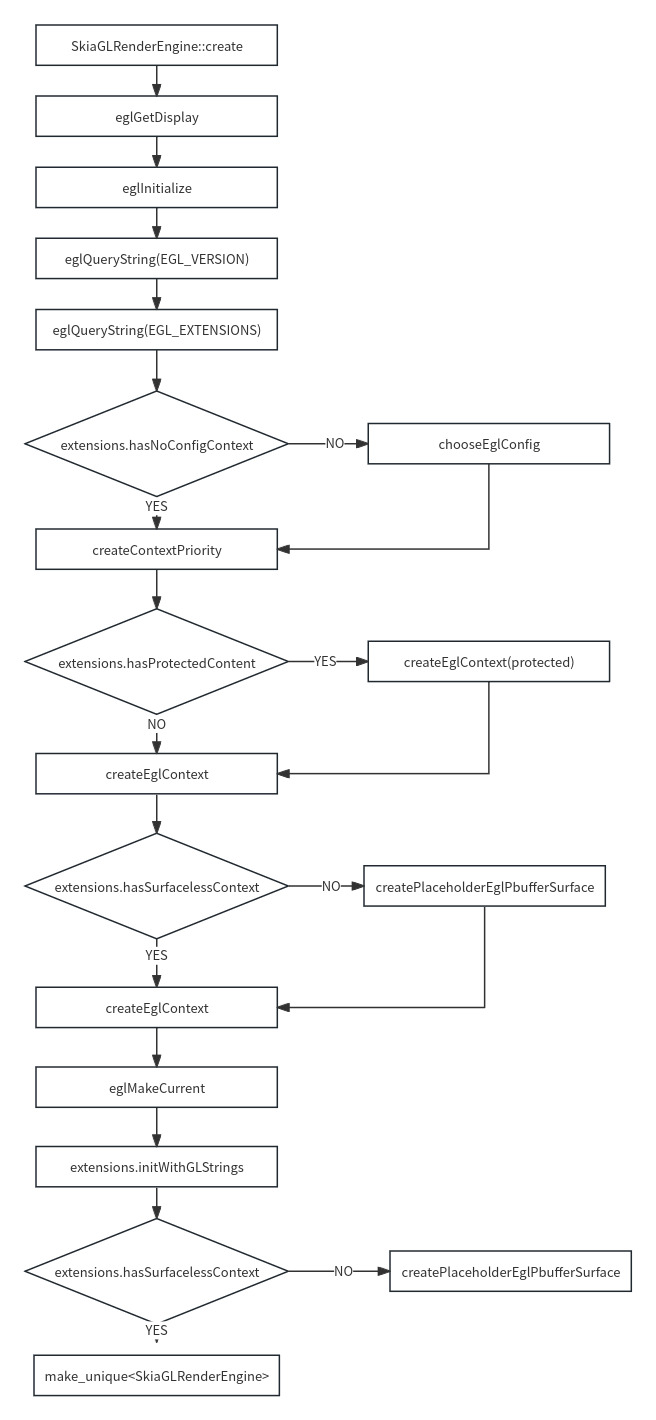
\includegraphics[width=0.35\textwidth]{skia_create过程.jpg}
  \caption{skiaRenderEngine创建时初始化EGL流程图}
\end{figure}

Android 2D渲染引擎默认使用的是skia,在SurfaceFlinger初始化过程中,会创建一个线程专门用于skia引擎的初始化并用于后续的图形绘制,
因此surfaceflinger初始化过程的关键是skia引擎的初始化。在SkiaGLRenderEngine::create时,
会依次执行eglGetDisplay获取EGL显示句柄,此句柄代表了要渲染的物理设备;eglInitialize初始化EGL环境,并获得EGL的主次版本号;
eglQueryString查询与当前显示连接相关的字符串信息,包括EGL版本信息、供应商版本信息以及支持的客户端API等,安卓还会使用EGL\_EXTENSIONS
获取有关安卓特性的拓展并初始化;使用createEglContext在EGL中创建 OpenGL ES 上下文;然后使用eglMakeCurrent将指定的渲染上下文和表面设置为当前的函数。

下面以eglInitialize为例,说明surfaceflinger是如何通过安卓的framework层的接口调用龙芯用户态驱动程序的。

\begin{figure}[h]
  \centering
  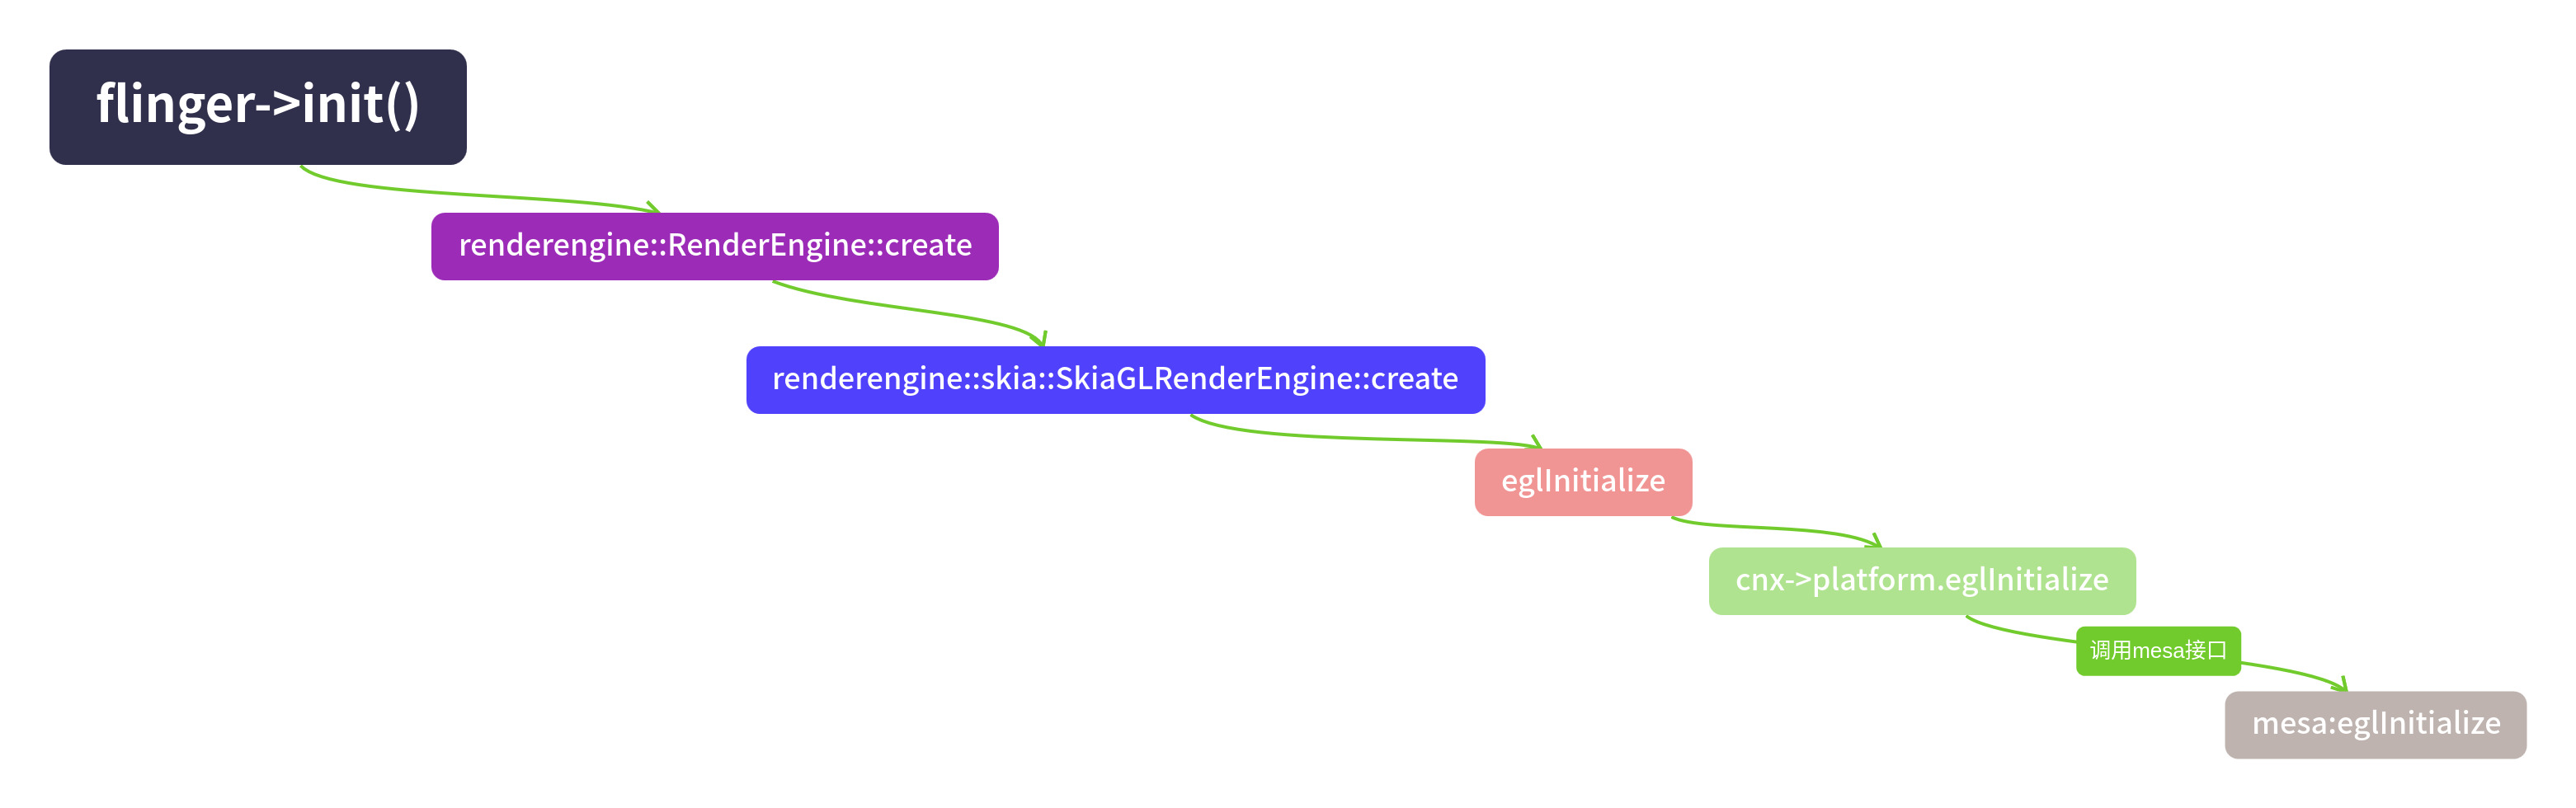
\includegraphics[width=0.8\textwidth]{flinger_egl初始化示意图.jpg}
  \caption{flinger驱动调用函数栈}
\end{figure}

首先是surfaceflinger初始化,调用flinger->init函数,根据PROPERTY\_DEBUG\_RENDERENGINE\_BACKEND宏判断使用渲染引擎的类型,可以是GLESRenderEngine
或SkiaGLRenderEngine,安卓中一般默认的都是SkiaGLRenderEngine,然后是引擎的create。调用eglInitialize,会使用LayerLoader::LoadLayers
中dlopen加载的libGLES\_mesa.so去初始化修饰的egl\_connection\_t结构体,调用gEGLImpl的接口,从而实现对龙芯用户态显卡驱动的调用。
GPU驱动的加载在Surfaceflinger的初始化过程中skia(2D渲染引擎)创建时进行加载,根据设置的驱动加载方式(本文使用的是dri2)
在eglInitialize时通过eglApi的接口调用mesa中的eglInitialize函数dri2\_initialize,从而实现mesa驱动的加载和初始化。

\section{龙芯安卓图形系统详细方案}
安卓使用的图形协议是深度定制的,而x11,wayland协议是运行在传统linux内核下的协议,因此龙芯现有的图形栈解决方案在安卓上并不完全适用。
并且由于Android多应用于ARM架构,而ARM与LoongArch架构的图形系统有较大差异,具体表现为ARM架构下的GPU没有独立显存\cite{Inki},而在LoongArch的内核中,需要
使用DRI框架来调用GPU,并且GPU有自己的独立显存。因此,首先需要解决的是在LoongArch架构下,Android系统中显存和系统内存分配映射的问题。AndroidX86\cite{AndroidX86}
很大程度上解决这个问题,该项目使用Mesa作为OpenGL ES实现,基于DRM和GEM实现了gralloc.drm.so模块,成功的使SurfaceFlinger在x86架构下运行并实现硬件加速\cite{XTYY201710015}。
但是Android自Q版本开始,为了提供图形性能和增强对硬件的支持,
对图形系统进行了重构与优化,至S版本稳定下来,中间迭代了4个API版本,在实现gralloc和HWC时需要考虑API的兼容性。具体表现为,引入了Gralloc2 API(至Android S版本Gralloc4稳定)和
HWC2,由于龙芯硬件的限制,HWC实际上使用的是hwcomposer1.0的实现,便不做过多讨论。以下将从mesa,HWC,gralloc简要说明需要完成的任务。

\subsection{内核驱动}
现使用安卓内核版本为5.10,由于龙芯gsgpu内核驱动属于闭源状态,尚未整合到已有的内核源码,采用的方案为驱动模块独立开发的方式,
这样设计有多个方面的好处,

一是为了适应多种方式加载驱动模块的需求,既可以通过加载/lib/modules/\$(kernel\_uname)下
的内核源码头文件实现在已有的系统上动态编译驱动模块并通过DKMS(Dynamic Kernel Module Support)加载,实现在已运行的系统上完成显卡内核驱动模块的安装;也可以通过静态编译,
指定静态的源码树的位置并编译生成可加载的.ko驱动文件。由于安卓主要采用的是静态内核模块(built-in or prebuilt kernel modules)方式来管理驱动,
不支持原生的DKMS,因此本课题采用的是静态编译的方式,在源码树之外编译.ko驱动文件,并在进入安卓系统后使用insmod方式加载.ko驱动文件。

二是为了适应多种内核版本的需求,现龙芯平台主流内核版本为4.19、5.5或6.6,而本课题使用的安卓内核版本为5.10,内核驱动涉及的接口多有变化。
而gpu/drm模块的接口变化较多,这是因为显示模块由于硬件设计上的变化,内核模块的代码需要不断进行调整和优化,以适应现代GPU设备和复杂内存管理的需求。
如表\ref{tab:内核4.19-5.10 drm接口变化}所示,仅从4.19到5.10,drm模块的接口变化已有48项之多,这些接口上的变化导致具体的内核驱动模块需要不断更新迭代,耗时耗力。
因此在原有的4.19内核版本驱动的基础上进行多版本适配,即可以动态识别内核驱动版本接口,是非常有意义的。

\begin{table}[h]
  \centering
  \caption{内核4.19-5.10 drm接口变化}
  \label{tab:内核4.19-5.10 drm接口变化}
  \begin{tabular}{lll}
    \toprule
    类型   &   名称  &变化时内核版本  \\
    \midrule
    变量 & DRIVER\_PRIME & 5.4 \\
    变量 & DRIVER\_IRQ\_SHARED & 5.1 \\
    函数 & drm\_sched\_stop & 5.1 \\
    函数 & drm\_fb\_helper\_fill\_info & 5.2 \\
    变量 & glob(ttm\_bo\_device\_init) & 5.0 \\
    函数 & ttm\_resource\_manager & 5.9 \\
    ... & ... & ... \\
    \bottomrule
  \end{tabular}
  \note{共计48项}
\end{table}

\subsubsection{多版本适配方案设计}
由于drm模块的接口变化为某个函数的增加或删除,部分结构体的属性变化,以及函数的参数变化。以空参数调用某个函数时,若函数相关实现已被删除,则测试代码\textbf{不会产生}编译错误,
仅会在链接时产生错误,而函数存在时,则会产生编译错误,将此种情况命名为function;若某个函数的形参不存在或者结构体或者结构体的某个属性不存在时,则测试代码\textbf{会产生}编译错误,
此种情况命名为type。这两种情况存在和不存在时目标对象时编译结果完全相反,结果判断如表\ref{tab:测试代码判断表}所示。针对不同实现缺失的情形,返回的编译结果完全相反。

\begin{table}[h]
  \centering
  \caption{测试代码判断表}
  \label{tab:测试代码判断表}
  \begin{tabular}{lll}
    \toprule
    类型   &   编译结果 & 函数\&属性\&参数是否存在    \\
    \midrule
    function & 不通过 & 存在 \\
    function & 通过 & 不存在 \\
    type & 通过 & 存在 \\
    type & 不通过 & 不存在 \\
    \bottomrule
  \end{tabular}
\end{table}

具体的方式为实现一个conftest.sh的脚本,假使该目标宏定义为DEF,如算法\ref{algo:algorithm1}所示,通过尝试编译测试代码,测试代码中引入已有的内核头文件,并按以下数种情况实现测试代码:

1.某函数实现删除或增加,假设目标测试函数为funcB,使用一个空返回值空形参的测试函数funcTest并调用无参数的目标函数,可视funcA的返回值情况选择是否设置funcB的返回值,
如算法\ref{algo:algorithm2}所示。

2.某函数实现的形参删除或增加,沿用1假设,添加调用funcB所需的参数,调用funcB并返回,如算法\ref{algo:algorithm3}所示。

3.某结构体的删除或增加,假设目标结构体类型为A,在funcTest中使用A的形参即可,如算法\ref{algo:algorithm4}所示。

4.某结构体中属性的删除或增加,沿用3假设,目标结构体的目标属性为c,使用offsetof(offsetof是一个 C语言的宏,
主要用于计算 结构体成员相对于结构体起始地址的偏移量)测试该结构体是否存在属性c,如算法\ref{algo:algorithm5}所示。

通过编译测试代码的结果(即是否生成中间代码.o文件)以及相应的类型(即function或者type)判断是否存在相关实现,并以此为基础生成相应的宏头文件,为GPU内核驱动的具体实现中提供判断基础。

\begin{algorithm}[h]
  \SetAlgoLined
  ...\;
  将测试代码重定向至conftest.c\;
  尝试编译conftest.c并忽略异常输出\;
  \eIf{存在conftest.o文件}{
    \eIf{类型为function}{
      显示未定义DEF并将其重定向至头文件\;
    }{
      显示已定义DEF并将其重定向至头文件\;
    }
  }{
    \eIf{类型为type}{
      显示已定义DEF并将其重定向至头文件\;
    }{
      显示未定义DEF并将其重定向至头文件\;
    }
  }
  \caption{编译检查测试函数}
  \label{algo:algorithm1}
\end{algorithm}

\begin{minipage}{0.45\textwidth}
  \begin{algorithm}[H]
    \SetAlgoLined
    \KwData{void}
    \KwResult{TypefuncB}
    TypefuncB funcTest(void){\\
      return funcB()\;
      or \;
      funcB()\;
    }
    \caption{测试代码示例1}
    \label{algo:algorithm2}
  \end{algorithm}
\end{minipage}
\hfill
\begin{minipage}{0.45\textwidth}
  \begin{algorithm}[H]
    \SetAlgoLined
    \KwData{arg1,arg2,...}
    \KwResult{TypefuncB}
    TypefuncB funcTest(Type1 arg1,Type2 arg2,...){\\
      return funcB(arg1,arg2,...)\;
    }
    \caption{测试代码示例2}
    \label{algo:algorithm3}
  \end{algorithm}
\end{minipage}

\begin{minipage}{0.45\textwidth}
  \begin{algorithm}[H]
    \SetAlgoLined
    \KwData{TypeA}
    \KwResult{void}
    void funcTest(TypeA a){\\
      return \;
    }
    \caption{测试代码示例3}
    \label{algo:algorithm4}
  \end{algorithm}
\end{minipage}
\hfill
\begin{minipage}{0.45\textwidth}
  \begin{algorithm}[H]
    \SetAlgoLined
    \KwData{void}
    \KwResult{int}
    int funcTest(void){\\
      return offsetof(struct B,c) \;
    }
    \caption{测试代码示例4}
    \label{algo:algorithm5}
  \end{algorithm}
\end{minipage}

\subsubsection{命令流管理模块}
\subsubsection{显示控制模块}
\subsubsection{转换表映射模块}
LG110内存模型

GPU 内存在物理上分为两个部分,
一部分是 GPU 本地的 VRAM 内存,另外一部分位于系统主存,也就是 GPU 的GTT 内存。GPU 的 VRAM 内存被映射到 CPU 的 PCI 地址空间中,而 GPU 的GTT 内存通过页表映射到系统主存上。
CPU可以通过PCI地址直接访问GPU的VRAM地址内存,而GPU的GTT内存实际上是系统内存,应用程序可以通过MMU将物理地址映射到用户地址空间再访问。
而GPU内部进行访问时,若GPU地址位于GTT内存时,通过DMA请求将数据异步传输到GPU。
\begin{figure}[h]
  \centering
  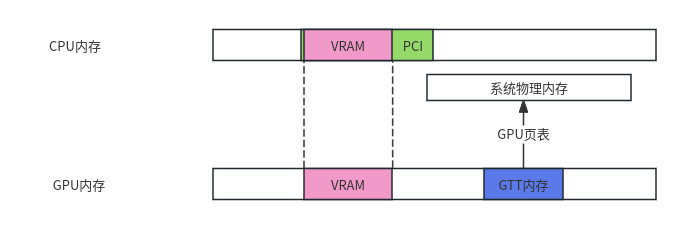
\includegraphics[width=0.8\textwidth]{LG110内存模型.jpg}
  \caption{LG110内存模型}
\end{figure}
转换表映射模块:
TTM(Translation Table Maps)适用于GPU内存管理的一部分,提供了对显存(VRAM)、主存、共享内存等不同类型内存的管理功能。
它通过一个通用的 API 提供内存分配、缓冲区对象管理和内存交换等功能,使得 GPU 驱动能够灵活管理图形资源。
TTM 需要实现的功能有:缓冲区对象(BO)创建与销毁、 内存管理与分配、内存驱逐和交换、内存访问控制、I/O 内存管理和缓冲区对象的绑定与解绑。
\begin{figure}[h]
  \centering
  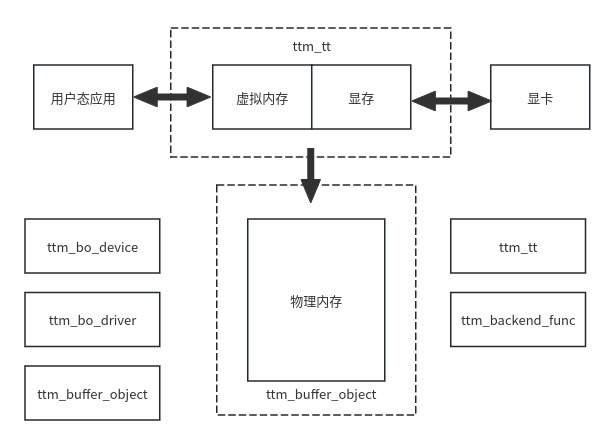
\includegraphics[width=0.8\textwidth]{DRM TTM结构.jpg}
  \caption{TTM主要对象}
\end{figure}

\subsection{mesa}
mesa使用的版本为18.3.6,而由于现有的安卓版本为12.0.0,安卓API版本为31对应的mesa版本为20.3.4,因此需要对现有的mesa的dri接口进行升级。并且由于安卓新的
编译方式Soong的加入,mesa目前最新的版本已经废弃了传统的mk编译方式,转而采用伪编译的方式。为考虑后续版本的兼容性,因此在现有的mesa18.3.6上采用伪编译的方法,
使用mesa原生的ninja编译方式,将生成的动态库文件添加到安卓目标生成目录中。此后,mesa库将被编译为libgallium\_dri.so以及libglapi.so。其中libgallium\_dri.so
用于支持DRI使得应用程序可以直接与GPU进行通信,绕过X服务器从而实现更高效的渲染;同时实现多个图形API,包括OpenGL,利用Gallium3D的架构来支持gsgpu的后端。而libglapi.so
则负责管理OpenGL API调用的分发,将调用路由到适当的实现,通常是后端的图形驱动程序并且处理OpenGL上下文的创建、管理和切换,确保正确的状态和资源在不同的渲染上下文中得到维护。
由此背景,可以分析得到以下数个方面。

\subsubsection{编译与构建适配}
由于mesa是一个开源的OpengGL实现,提供了多种GPU硬件的驱动支持,因此代码提交量极大。而mesa原生编译框架使用的是ninja,而Android中使用的是Makefile,直接编译生成目标动态库文件,
与原生ninja并无关系,因此需要使用伪编译框架去生成动态库文件,即用cross-compile配置mesa交叉编译脚本aosp-cross,再使用原生ninja编译规则生成目标安装目录install,
将生成的目标文件安装到AOSP编译框架指定的vendor分区,为后续龙芯mesa版本提供支持。

mesa编译框架如图\ref{fig:mesa编译框架},AOSP编译框架会自动监测所有的Android.mk并编译,Android.mk会调用mesa3d\_cross.mk生成aosp\_cross的mesa交叉编译规则,
按照mesa原生的编译规则生成安装目录install,再将目标动态库文件安装到指定的vendor分区。
\begin{figure}[h]
  \centering
  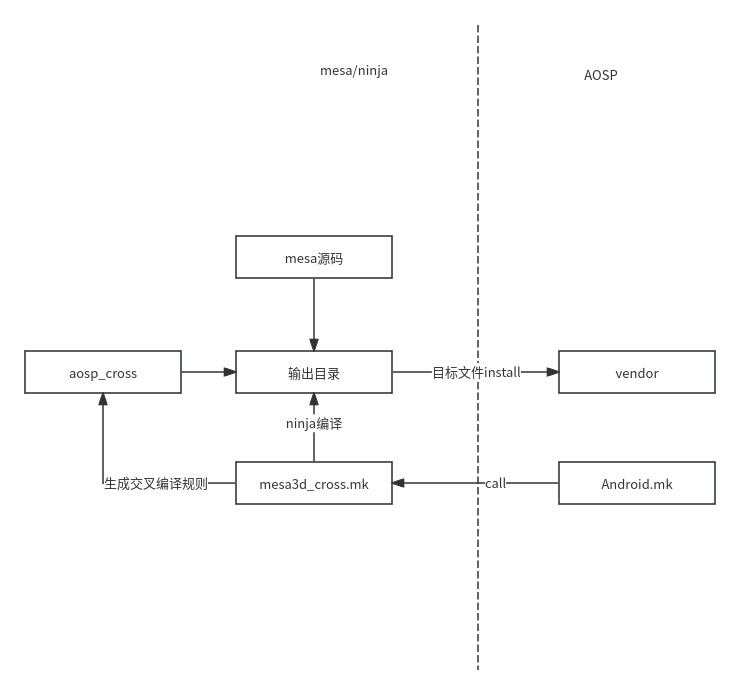
\includegraphics[width=0.8\textwidth]{mesa编译框架.jpg}
  \caption{mesa编译框架}
  \label{fig:mesa编译框架}
\end{figure}

% \subsubsection{图形 API 支持}
% 打通GPGPU后端支持Gallium3D的通路,确保 OpenGL 的核心功能集成到龙芯平台,确保API 的正确性。

% \subsubsection{性能优化}
% 针对龙芯架构的特点,优化 Mesa 的编译选项以提升性能。
% 针对 Gallium3D 后端渲染效率的优化,包括批处理、资源管理和 API 调用路径。

\subsubsection{mesa目标安装文件说明}
% 目前龙芯LG110显卡用户态实现主要是在Mesa上,Mesa是集成了OpenGL、OpenGL ES和Vulkan等3D图形API支持的开源图形库\cite{mesa3d}。
% 由安卓12的兼容性文档来看,安卓12要求硬件必须满足OpenGL ES 1.1以及2.0的实现,并且需要支持EGL\_KHR\_image、EGL\_ANDROID\_image\_native\_buffer、
% EGL\_ANDROID\_recordable等等相关拓展。目前LG110已满足相关兼容性标准的最低要求,可以作为Android图形系统运行的硬件基础。
% 另外,由于Android系统主要用于arm架构,而arm架构下的GPU多数没有自己的独立显存,系统服务SurfaceFlinger申请的帧缓存属于系统内存,而在本课题中,LoongArch架构下,
% GSGPU有自己的专属独立显存。因此首先要解决的是如何让SurfaceFlinger能够在LoongArch架构下运行,同时由于SurfaceFlinger是基于OpenGL ES标准实现的,所以需要
% 有能在LoongArch架构下。????

安卓需要使用数个Mesa编译生成的动态库文件:

libEGL.so.1.0.0,是一个用于处理 EGL (Embedded-System Graphics Library) 接口的共享库,为 OpenGL ES 或 OpenVG 提供了对底层图形设备的抽象;

libGLESv1\_CM.so.1.1.0,是一个用于实现 OpenGL ES 1.x(特别是 OpenGL ES 1.1 和 OpenGL ES 1.0)功能的共享库),负责将 OpenGL ES 1.x 请求转换为 GPU 可执行的指令;

libGLESv2.so.2.0.0,是一个提供 OpenGL ES 2.x 功能的共享库,用于支持 OpenGL ES 2.x(及以上版本)的图形渲染,提供了着色器的支持等;

libglapi.so.0.0.0,提供 OpenGL API 调用 的代理功能,使得 OpenGL 函数调用可以通过动态链接的方式,调用不同的 OpenGL 实现库;

以及为了支持gralloc的功能需要安装的libgbm\_mesa.so.1.0.0,提供GBM(Generic Buffer Management)接口的实现,主要用于管理图形缓冲区;

libgallium\_dri.so,提供了 Gallium 框架下的 Direct Rendering Infrastructure (DRI) 驱动程序实现。

上述数个动态库文件,会被安装到对应的供应商(vendor)分区,以供系统服务(如SurfaceFlinger)等使用。

\subsection{Android HAL层实现}

\subsubsection{硬件混合渲染模块}
%每个厂商hwc实现可能不同如nxp,rockchip,drm-hwc,ranchu,也有很多厂商实现是闭源的如nxp,而谷歌的drm-hwc,ranchu是开源的
由于没有硬件HWComposer,因此SurfaceFlinger的画面合成过程是基于OpenGL ES完成的,是使用client模式合成,因此hwcomposer.drm\_minigbm.so只是一个符合HWComposer1.0接口标准的软件实现,
并不是硬件HWComposer的驱动程序。它在进行画面更新时实际上会先atomic设置plane的状态,实际上就是调用libdrm的drmModeAtomicAddProperty接口,用于设置显示设备的相关属性,然后atomic向
底层drm系统提交显示信息,也就是调用libdrm的drmModeAtomicCommit接口,更改显示设备的配置。

\subsubsection{图形缓存分配模块}
由于Android系统主要用于arm架构,而arm架构下的GPU多数没有自己的独立显存,系统服务SurfaceFlinger申请的帧缓存属于系统内存,而在本课题中,LoongArch架构下,
GSGPU有自己的专属独立显存。因此首先要解决的是如何让Android的SurfaceFlinger能够在LoongArch架构下运行,而SurfaceFlinger依赖的缓冲区管理的HAL实现就是gralloc。
依照Android 12的gralloc标准,gralloc模块接口定义有两部分,分别是mapper和allocator,
位于AOSP源码结构下的hardware/interface/graphic/mapper以及hardware/interface/graphic/allocator,
其中定义了缓冲区的描述符的数据结构,创建、导入、释放缓冲区对象等。本课题按照hal文件定义的接口实现了一个绑定式图形缓存分配器。

gralloc模块的HAL服务有绑定式(Binderized )也有直通式(Passthrough),区别在于,直通式会被编译成.so库文件,为system和vendor分区的进程和应用在运行时动态加载调用,两者是在
同一进程中,而绑定式会被编译成一个可独立运行的服务,类似于一个守护进程,然后相关服务进程或应用会通过HwBinder的IPC(进程间通信)方式来调用,是在两个独立的进程中。绑定式是Google
在Android8.0时,为了方便升级系统框架所做的解耦技术。而绑定式又有默认直通式实现(defaultPassthroughServiceImplementation)以及 注册成服务(RegisterAsService)
两种类型,本课题采用的是第二种。在具体的实现上,采用VINTF Fragments为本模块创建清单并与相应的hal相关联,并且需要设置rc文件并安装到/vendor/etc/init目录下,为init进程初始化
提供执行依据(init进程会在加载init.rc主目录后立即加载/system/etc/init、/vendor/etc/init、/odm/etc/init等相关目录中的文件)。

\begin{figure}[h]
  \centering
  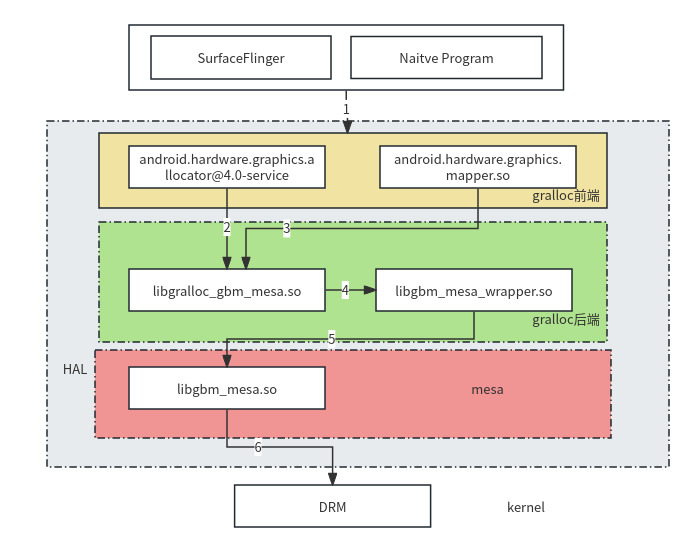
\includegraphics[width=0.8\textwidth]{gralloc调用栈.jpg}
  \caption{gralloc调用栈}
  \label{fig:gralloc调用栈}
\end{figure}

Android自身提供了共享内存的机制,native\_handle\_t是一个用于描述缓冲区的结构体,可以在进程之间传递缓冲区信息,gralloc\_handle\_t是Android 图形缓冲区分配器(Gralloc)中的句柄结构,
它继承自 native\_handle\_t,用于管理共享图形缓冲区。gralloc\_handle\_t这一特性需要libdrm的支持,最低版本需要2.4.97之后才支持此特性,目前龙芯已有的libdrm的解决方案已有2.4.97,
满足相关支持。然后gralloc\_handle\_t图形缓冲区的创建需要显卡驱动的GBM框架(mesa提供的通用缓冲区管理接口)提供支持,然后GBM会调用直接渲染框架(DRI)的接口作为后端,与内核进行交互。
如图\ref{fig:gralloc调用栈}所示,Android系统上层应用程序在需要使用图形缓存时,使用路径1通过IPC(Inter-Process Communication)跨进程通信向gralloc守护进程申请图形缓存,
然后allocator和mapper会通过路径(2-3)调用gralloc后端封装的缓冲区操作函数(函数具体见\ref{tab:gralloc模块后端接口表}),这些操作函数通过路径4调用gbm封装层wrapper,该wrapper封装了
一组与GBM对象操作相关的函数(详细接口见\ref{tab:gbm封装层接口表}),通过路径5直接调用mesa的gbm实现,而gbm会通过路径6内核DRM接口drmIoctl向内核申请创建缓冲区。

\begin{table}[h]  
  \centering
  \caption{gralloc模块后端接口表}
  \label{tab:gralloc模块后端接口表}
  \begin{tabular}{ll}
    \toprule
    接口名  & 作用\\
    \midrule
    init\&close & 驱动程序的初始化和关闭 \\
    bo create & 创建缓冲区对象(BO)的函数,实现内存分配和初始化 \\
    bo destroy & 销毁缓冲区对象的函数,负责释放已分配的内存 \\
    bo import & 导入缓冲区对象的函数,允许将外部缓冲区导入到 GBM 管理的缓冲区中 \\
    bo map & 映射缓冲区对象的函数,使得 CPU 可以访问 GPU 分配的内存 \\
    bo unmap & 解除映射缓冲区对象的函数,释放 CPU 对缓冲区的访问 \\
    bo get plane fd & 获取缓冲区对象平面的文件描述符。\\
    bo get map stride & 获取缓冲区对象的映射跨度。 \\
    resolve format and use flags & 解析格式和使用标志的函数,用于确定缓冲区对象的数据格式及其相关标志 \\
    \bottomrule
  \end{tabular}
  \note{}
\end{table}

\begin{table}[h]  
  \centering
  \caption{gbm封装层接口表}
  \label{tab:gbm封装层接口表}
  \begin{tabular}{ll}
    \toprule
    接口名  & 作用\\
    \midrule
    get gbm format & 获取与设备兼容的 GBM 格式 \\
    dev create/destroy & 创建或销毁 GBM 设备 \\
    alloc & 分配一个 GBM 缓冲区 \\
    import & 导入外部的 GBM 缓冲区 \\
    free & 释放已经分配的 GBM 缓冲区 \\
    map & 将 GBM 缓冲区映射到当前进程的地址空间 \\
    unmap & 解除 GBM 缓冲区的映射 \\
    \bottomrule
  \end{tabular}
  \note{}
\end{table}


1.gbm包装模块
用于在使用 Mesa 和 GBM(Generic Buffer Management)时对显存缓冲区(BO,Buffer Object)进行创建、映射、导入和销毁的操作。它通过封装与 GBM API 的交互,
简化了底层内存管理,并与 Android 环境中的驱动配合。实现了以下4个功能模块:
\textbf{缓冲区分配与管理}:缓冲区可用于多种渲染操作

\textbf{跨平台支持}:用于纹理处理等操作

\textbf{优化内存访问}:表示与软件处理相关

缓冲区分配与管理: 通过封装 GBM 的创建、导入、映射和销毁操作,实现了对缓冲区对象的管理,方便与其他模块进行交互。

跨平台支持: 代码通过不同的条件编译支持在多种架构(如 x86\_64、ARM 等)上的适配,特别是不同平台上缓冲区的对齐和映射步长差异。

优化内存访问: 在导入缓冲区时,确保正确的映射步长(map\_stride)处理,避免不同驱动和硬件上的差异,保证高效内存访问。

调试与日志: 通过 ALOGE 和 ALOGV 等宏进行调试输出,帮助开发人员调试 GBM 缓冲区分配和管理过程。

此外由于Android平台有自己的HAL\_PIXEL\_FORMAT格式,而DRM有自己的DRM\_FORMAT格式因此需要进行格式转换,所以按照mesa的标准,可以得出如下的格式转换表\ref{tab:HAL格式转换表},
此处仅列出一些常用和目前课题硬件支持的图形格式。

\begin{table}[h]  
  \centering
  \caption{HAL格式转换表}
  \label{tab:HAL格式转换表}
  \begin{tabular}{lll}
    \toprule
    HAL\_PIXEL\_FORMAT & DRM\_FORMAT  & value\\
    \midrule
    HAL\_PIXEL\_FORMAT\_RGBA\_8888 & DRM\_FORMAT\_ABGR8888 & 1\\
    HAL\_PIXEL\_FORMAT\_RGBX\_8888 & DRM\_FORMAT\_XBGR8888 & 2\\
    HAL\_PIXEL\_FORMAT\_RGB\_888 & DRM\_FORMAT\_BGR888 & 3\\
    HAL\_PIXEL\_FORMAT\_RGB\_565 & DRM\_FORMAT\_RGB565 & 4\\
    HAL\_PIXEL\_FORMAT\_BGRA\_8888 & DRM\_FORMAT\_ARGB8888 & 5\\
    ... & ...&...\\ 
    \bottomrule
  \end{tabular}
  \note{}
\end{table}

gralloc模块分为HAL服务实现(可以称为gralloc前端),gbm接口实现模块和gbm包装层(可以称为gralloc后端)。前端已有部分开源代码实现,因此可以使用公共层的代码,
相应的,本课题只需要实现后端代码,即gbm的接口对接和封装等。

由于上层应用是通过gralloc获取实际的图像缓冲描述句柄,而由于不同进程使用图像缓冲区的目的不同。如UI进程是为了渲染画面并传送给SurfaceFlinger进行合成,而SurfaceFlinger是
要在自己的缓冲区上合成帧画面并送显,因此图像缓冲区的类型往往不同。

\textbf{BO\_USE\_RENDER\_MASK}:缓冲区可用于多种渲染操作

\textbf{BO\_USE\_TEXTURE\_MASK}:用于纹理处理等操作

\textbf{BO\_USE\_SW\_MASK}:表示与软件处理相关

\textbf{BO\_USE\_GPU\_HW}:与GPU硬件加速相关

\textbf{BO\_USE\_NON\_GPU\_HW}:表示与非GPU硬件加速相关

\textbf{BO\_USE\_HW\_MASK}:表示与所有硬件相关

%  缓冲区对象buffer object数据结构
% 而gbm接口实现模块需要完成一些与硬件特性相关的接口函数,如:

% \textbf{init\&close}:驱动程序的初始化和关闭

% \textbf{bo create}:创建缓冲区对象(BO)的函数,实现内存分配和初始化

% \textbf{bo destroy}:销毁缓冲区对象的函数,负责释放已分配的内存

% \textbf{bo import}:导入缓冲区对象的函数,允许将外部缓冲区导入到 GBM 管理的缓冲区中。

% \textbf{bo map}:映射缓冲区对象的函数,使得 CPU 可以访问 GPU 分配的内存。

% \textbf{bo unmap}:解除映射缓冲区对象的函数,释放 CPU 对缓冲区的访问。

% \textbf{bo get plane fd}:获取缓冲区对象平面的文件描述符。在多平面的缓冲区(如YUV格式图像)中,平面文件描述符用于访问每个平面数据。

% \textbf{bo get map stride}:获取缓冲区对象的映射跨度。不同的缓冲区格式可能具有不同的内存布局(例如行对齐),stride 描述了每行数据的字节数

% \textbf{resolve format and use flags}:解析格式和使用标志的函数,用于确定如何使用缓冲区对象的数据格式及其相关标志

缓冲区对象buffer object数据结构
其中在创建缓冲区时会首次获取并初始化显卡驱动,如\ref{algo:gralloc初始化显卡驱动},

\begin{algorithm}[H]
  \SetAlgoLined
  \KwData{driver}
  \KwResult{shared\_ptr<GbmMesaDriver>}
  init\_driver(){\\
    ...
    遍历所有可用的DRM设备节点并获取相应的文件描述符fd\;
    加载wrapper的动态库\;
    调用gbm后端和DRM设备的文件描述符fd创建驱动\;
    ...\;
  }
  \caption{gralloc初始化显卡驱动}
  \label{algo:gralloc初始化显卡驱动}
\end{algorithm}

以bo\_create为例,首先初始化alloc\_args作为gbm后端调用的参数,根据输入的参数对width、height进行对齐处理,然后使用wrapper封装的gbm接口,使用gbm\_bo\_create创建
一个新的缓冲区对象bo,以bo作为参数以此调用gbm\_bo\_get\_fd获取缓冲区对象的文件描述符、gbm\_bo\_get\_stride获取缓冲区对象的步长、gbm\_bo\_get\_modifier获取缓冲区对象的格式修饰符,
并在上述步骤完成后因此此时可以通过文件描述符对缓冲区进行处理,因此销毁gbm缓冲区对象及时释放资源,如图\ref{fig:alloc过程}

\begin{figure}[h]
  \centering
  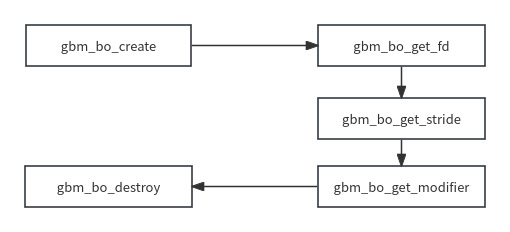
\includegraphics[width=0.8\textwidth]{alloc过程.jpg}
  \caption{alloc过程}
  \label{fig:alloc过程}
\end{figure}

\begin{algorithm}[H]
  \SetAlgoLined
  \KwData{gralloc\_buffer\_descriptor,native\_handle\_t}
  \KwResult{int32\_t}
  allocate(){\\
  DRM驱动初始化检查\;
  ... \\
  Hal格式与DRM格式检查\;
  Driver->allocate\;  \tcp{调用驱动的allocate方法} 
  句柄转换native\_handle\_t 转换成gralloc\_handle\_t\;
  outHandle设置结果输出\;
  }
  \caption{allocate}
  \label{algo:allocate}
\end{algorithm}

drmformat转换、回调框架说明、gralloc直通式等

依据硬件的设计可以选择在初始化时是否使用tiled等模式进行访存优化,提供更灵活的驱动交互方式。

\subsection{硬件适应性修改}
由于龙芯显卡 LG110 的存储管理单元(Memory Management Unit, MMU)采用页式管理来处理 GPU 所使用的内存,
所有内部功能模块均使用虚拟地址。在连接到内部网络之前,这些地址需要经过转换。当前,MMU 设计了三级页表结构,且页大小(page size)为 16KB。
然而,Android 12 尚未支持 16KB 的页大小。这意味着需要对以下几个方面进行修改:

\textbf{Bionic 库}:需要在 Bionic 中调整页面数据结构,以支持 16KB 的页大小。

\textbf{安卓通用内核文件系统}:在内核的文件系统(如ext4、super和f2fs)中添加对 16KB 页大小的支持。

\textbf{AOSP部分系统服务}:在 AOSP 中的部分系统服务中也需添加相应的支持。

具体实现方法是使用内联函数 page\_size() 来获取内核中的页大小,从而实现对多种页面大小的兼容。这种改动将确保龙芯显卡的 MMU 
能够高效地与 Android 系统和应用程序进行集成,提供更好的性能和兼容性。

% \subsection{内核编译\&bionic\&部分系统服务修改说明}

\textbf{内核编译}:本课题所使用的内核是安卓通用内核5.10,因此在编译时需要添加安卓特性相关的驱动支持如ASHMEM、BINDERFS、BINDERIPC等,
虚拟内存管理使用三级页表,页表大小为16Kb。将f2fs模块的相关的宏定义做适应性调整。
详见表\ref{tab:f2fs模块修改说明}。以此为基础,对f2fs模块中所有依赖这几个宏的相关实现进行修改。
\begin{table}[h]
  \centering
  \caption{f2fs模块修改说明}
  \label{tab:f2fs模块修改说明}
  \begin{tabular}{lll}
    \toprule
    宏名   &   原有  &改动  \\
    \midrule
    F2FS\_MAX\_LOG\_SECTOR\_SIZE & 12 & PAGE\_SHIFT \\
    F2FS\_LOG\_SECTORS\_PER\_BLOCK & 3 & PAGE\_SHIFT - 9 \\
    F2FS\_BLKSIZE & 4096 & PAGE\_SIZE \\
    F2FS\_BLKSIZE\_BITS & 12 & PAGE\_SHIFT \\
    \bottomrule
  \end{tabular}
  \note{}
\end{table}

\textbf{bionic\&部分系统服务修改:}这两个部分的适配的动机与内核类似,具体实现可以在bionic/libc/platform/bionic/page.h中实现一个内联page\_size()的函数用以实现从内核
中动态获取页表大小,并以此为适配有使用PAGE\_SIZE为4k相关的服务,累积完成40余处的修改。这个函数实现是用getauxval来获取与进程相关的辅助值(auxiliary vector values),而
辅助向量是内核传递给程序的额外信息,通常是在程序启动时传递给它的,用于提供关于系统环境的各种信息。AT\_PAGESZ就是辅助向量常量之一,用于查询系统的页面大小,如算法\ref{algo:获取内核页面大小}
同时,由于Android12中有大量的系统服务依然在使用PAGE\_SIZE宏,因此对相关系统服务做一些适应性修改在所难免,如图\ref{fig:androidS 16k适配改动图}
\begin{algorithm}[H]
  \SetAlgoLined
  \KwData{void}
  \KwResult{size\_t}
  inline size\_t page\_size(){\\
  \eIf{PAGE\_SIZE已定义}{
    return PAGE\_SIZE\;
  }{
    size = getauxval(AT\_PAGESZ)\\
    return size\;
  }
  }
  \caption{获取内核页面大小}
  \label{algo:获取内核页面大小}
\end{algorithm}

\begin{figure}[h]
  \centering
  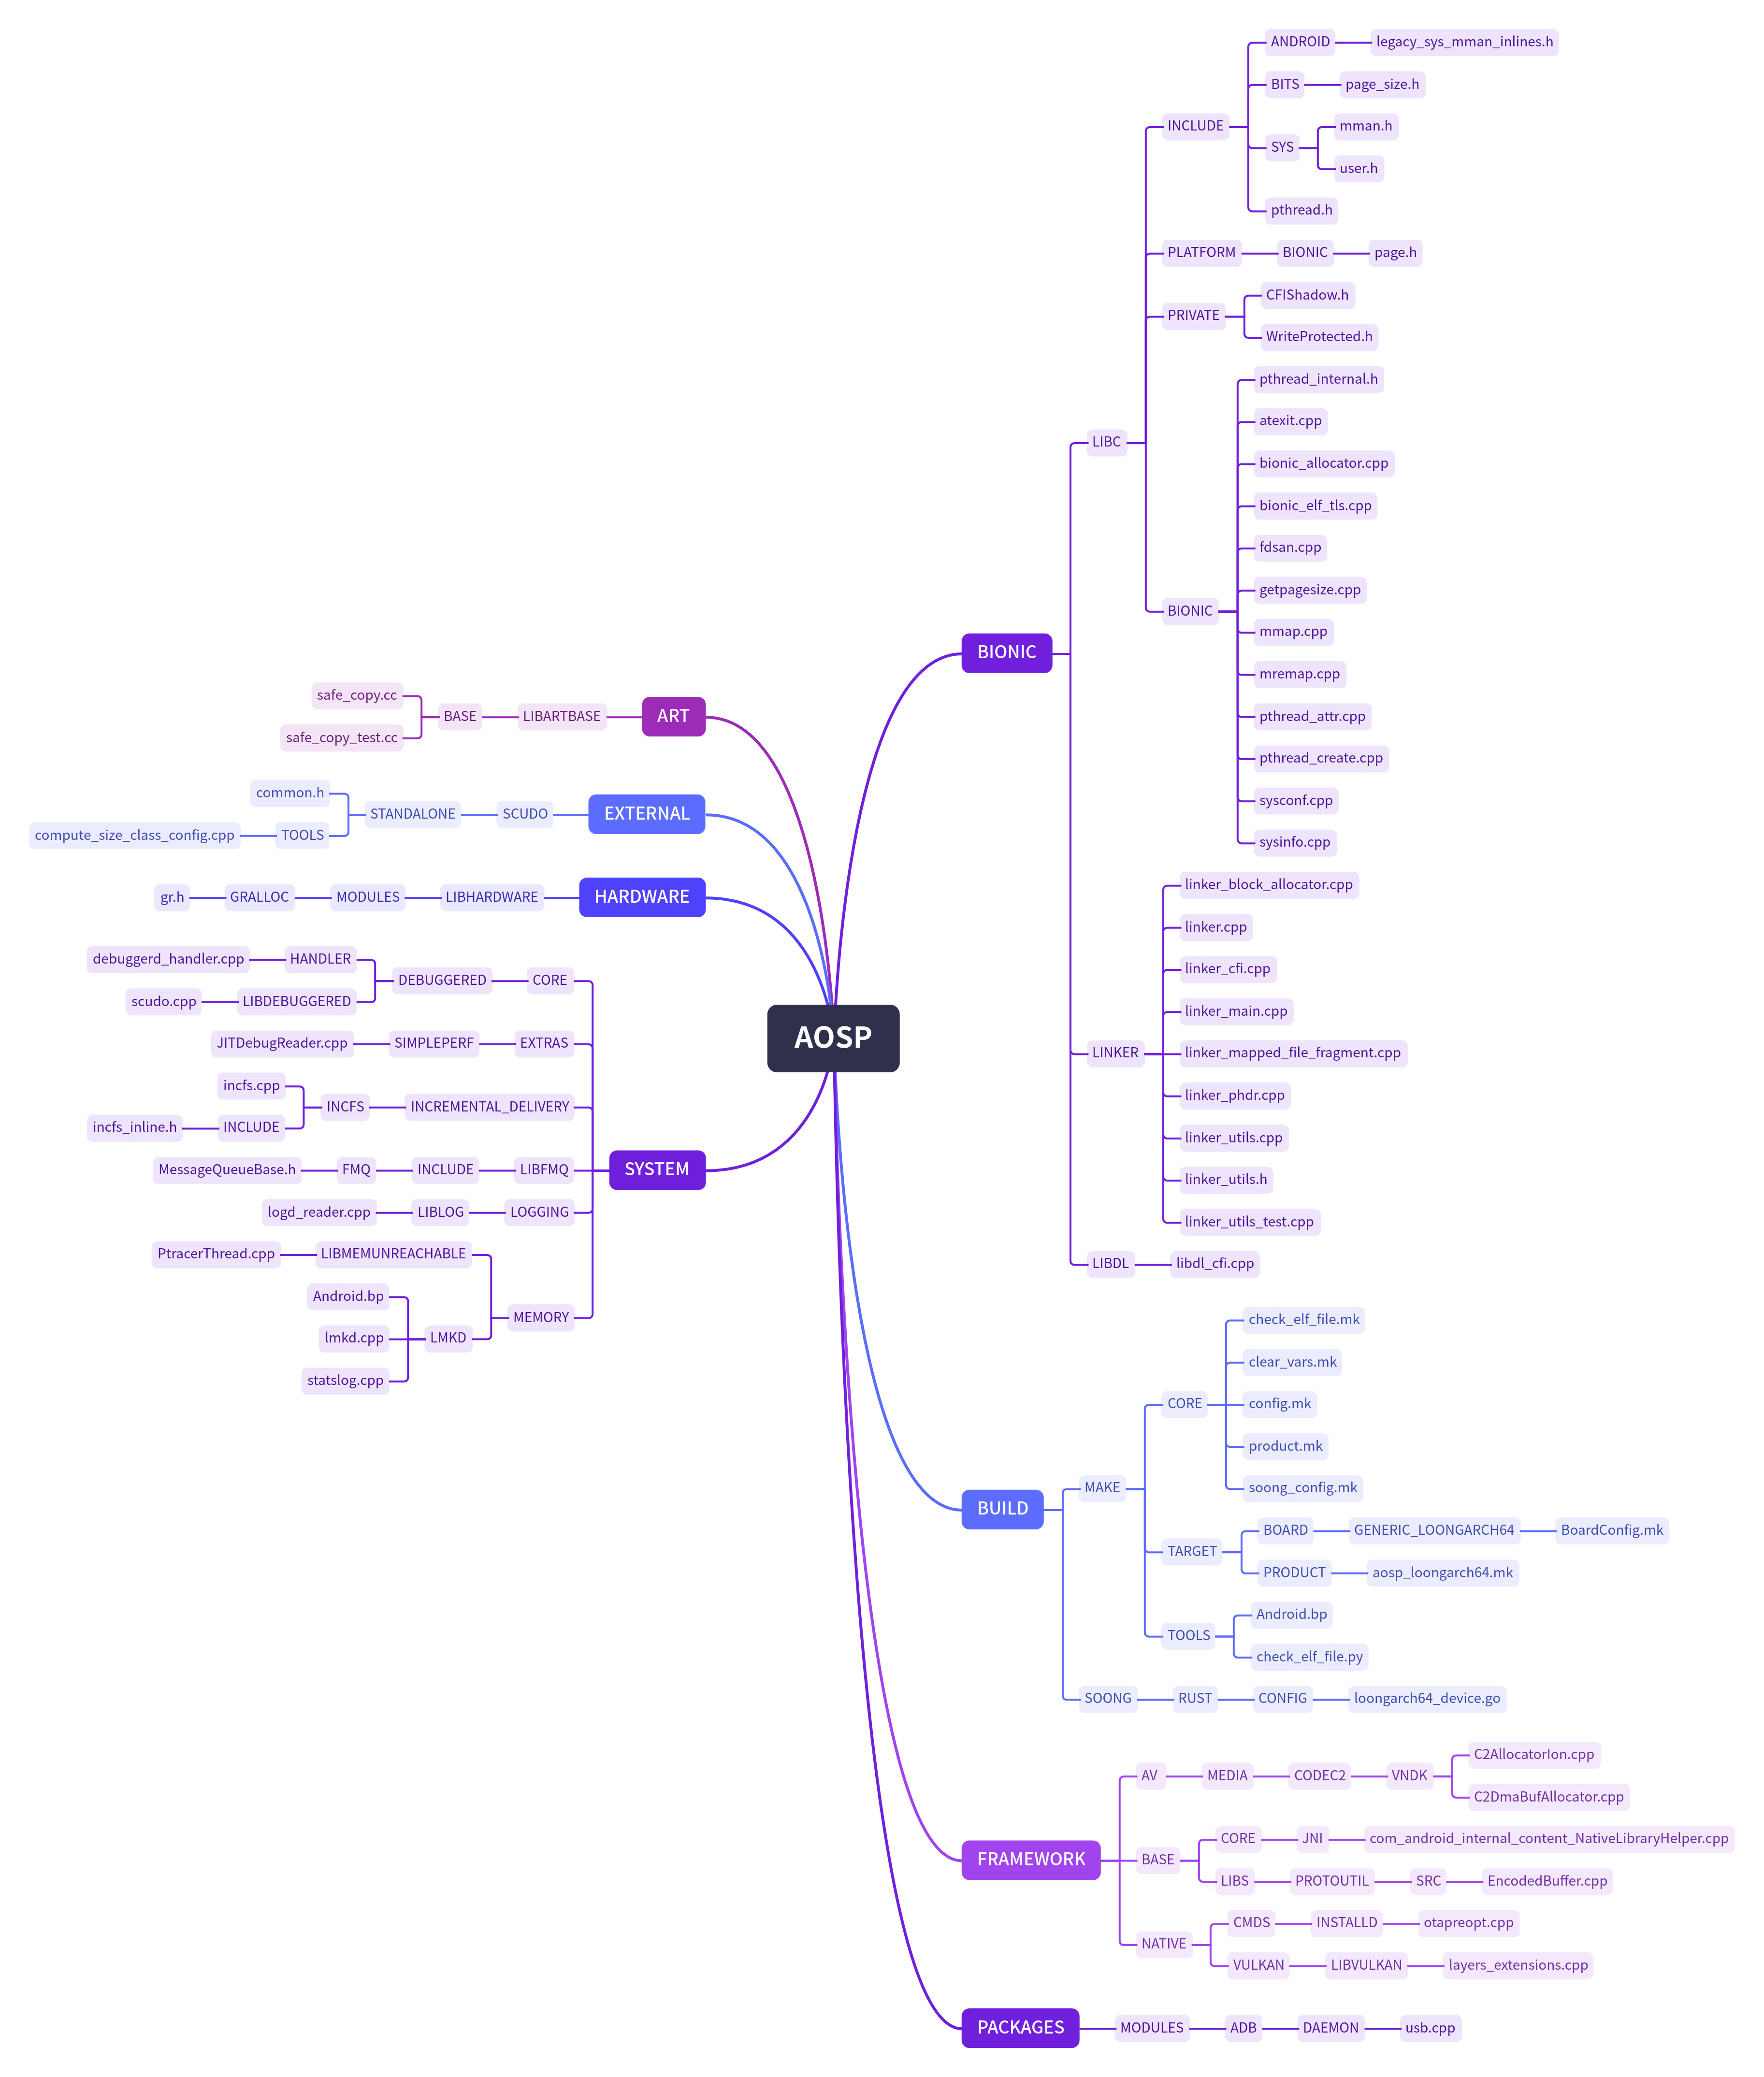
\includegraphics[width=0.8\textwidth]{androidS 16k适配改动图.jpg}
  \caption{androidS 16k适配改动图}
  \label{fig:androidS 16k适配改动图}
\end{figure}




% 字段名	对应的函数	功能描述
% name	"gsgpu_common"	模块的名称,通常用于标识该模块或打印调试信息。
% early_init	gsgpu_common_early_init	早期初始化函数,模块初始化前需要做的一些准备工作。
% late_init	gsgpu_common_late_init	后期初始化函数,在其他初始化完成后执行的工作。
% sw_init	gsgpu_common_sw_init	软件部分的初始化函数,通常用于分配内存、初始化数据结构等。
% sw_fini	gsgpu_common_sw_fini	软件部分的清理函数,用于释放资源、销毁数据结构。
% hw_init	gsgpu_common_hw_init	硬件部分的初始化函数,负责配置硬件寄存器或启动硬件功能。
% hw_fini	gsgpu_common_hw_fini	硬件部分的清理函数,负责关闭硬件功能或恢复硬件状态。
% suspend	gsgpu_common_suspend	挂起函数,通常在系统进入睡眠模式(如 S3)时调用,用于保存硬件状态。
% resume	gsgpu_common_resume	恢复函数,通常在系统从睡眠模式恢复时调用,用于恢复硬件状态。
% is_idle	gsgpu_common_is_idle	判断模块是否处于空闲状态的函数,通常用于调试或节能管理。
% wait_for_idle	gsgpu_common_wait_for_idle	等待模块进入空闲状态的函数,通常用于保证操作完成后再进行后续操作。
% soft_reset	gsgpu_common_soft_reset	软复位函数,用于在某些情况下重置模块,而无需对整个系统进行硬复位。
% \subsection{gralloc}




% 1. Allocator
% Allocator 负责内存的分配和释放,主要功能包括:

% 内存分配:
% 分配一块合适大小的内存区域,通常用于图形缓冲区(如帧缓冲、纹理等)。
% 格式支持:
% 支持多种像素格式(如 RGBA、YUV 等),确保分配的内存符合所需的格式和对齐要求。
% 内存管理:
% 管理可用内存的状态,跟踪已分配和未分配的内存区域,确保内存的高效使用。
% 性能优化:
% 通过优化内存分配策略(如缓存机制、批量分配等),提高图形性能。
% 2. Mapper
% Mapper 负责内存的映射和访问,主要功能包括:

% 地址转换:
% 将分配的内存地址转换为应用程序可用的地址,确保应用能够正确访问相应的内存区域。
% 映射和解除映射:
% 提供映射和解除映射的功能,允许应用在需要时将内存映射到其地址空间,使用完毕后解除映射。
% 共享内存管理:
% 支持不同进程之间共享内存,通过 Mapper,多个应用能够高效地访问同一块内存,减少内存复制的开销。
% 权限控制:
% 管理对内存的访问权限,确保只有经过授权的进程能够访问特定的内存区域。

% __DRI_IMAGE_PRIME_LINEAR_BUFFER
% front_rendering_usage __DRI_IMAGE_USE_FRONT_RENDERING 
% 两个扩展新特性可以写一写
% 1. EGL_EXT_image_dma_buf_import
% 功能:允许从 DMA-BUF 导入图像,以实现跨设备的缓冲区共享。
% 应用场景:在多 GPU 系统或使用不同硬件加速的情况下,支持高效的缓冲区共享。
% 2. EGL_ANDROID_image_native_buffer
% 功能:提供对 Android 原生图像缓冲区的支持,允许将图像直接与 Android 的图形系统进行交互。
% 应用场景:用于 SurfaceFlinger、硬件加速的视频播放和图形应用中。
% 3. EGL_ANDROID_surface_texture
% 功能:允许将 SurfaceTexture 用作 EGL 表面,使得 OpenGL ES 能够与 Android 的 SurfaceTexture 直接交互。
% 应用场景:用于实现视频和动画的优化渲染。
% 4. EGL_ANDROID_native_fence_sync
% 功能:支持在图形操作中使用本地栅栏同步机制,以提高 GPU 的并行处理能力。
% 应用场景:在需要同步多个 GPU 操作时提高性能。
% 5. EGL_KHR_create_context
% 功能:允许创建带有特定属性的上下文,增强了对不同版本的 OpenGL ES 的支持。
% 应用场景:为应用程序提供灵活性,以选择合适的 OpenGL ES 版本和功能。
% 6. EGL_EXT_image_gl_colorspace
% 功能:支持不同颜色空间的图像处理,以增强图形的表现力。
% 应用场景:在色彩管理和图像处理应用中使用。
% 7. EGL_KHR_swap_buffers_with_damage
% 功能:允许仅交换需要更新的缓冲区部分,提高交换的效率。
% 应用场景:在需要减少屏幕刷新时提高性能,特别是动态内容的应用。
% 8. EGL_KHR_partial_update
% 功能:支持部分更新 EGL 表面,允许只刷新屏幕的一部分。
% 应用场景:在需要频繁更新部分图像的应用中提高效率



% 安卓的gralloc负责管理图形内存的分配和共享,主要组件包括Allocator,Mapper以及BufferQueue。
% 在API29之后可使用cros grralloc与EGL结合,为gbm(General Buffer Manger)添加支持前渲染的能力。

% 安卓内核编译
%   gsgpu内核驱动编译
% mesa驱动层api兼容方案
% minigbm gsgpu后端接口实现
% 移植兼容方案
%   mesa伪编译代码实现
  %gsgpu内核驱动层多版本兼容方案

% \section{内核态驱动支持}
% gsgpu驱动 ttm,gem,vram
